\documentclass{beamer}
% \usepackage{animate}
\usepackage{multimedia}
\usepackage[english,russian]{babel}

\usepackage{pgfpages}
\setbeameroption{show notes on second screen}
%https://tug.ctan.org/macros/latex/contrib/beamer/doc/beameruserguide.pdf

\usepackage[T2A]{fontenc}
\usepackage[utf8]{inputenc}

\setbeamertemplate{caption}[numbered]

\usetheme{CambridgeUS}
\usecolortheme{dolphin}


\title[Физические аспекты]{Физические аспекты в моделях освещения}
\author[Быковских Д.А.]{Быковских Дмитрий Александрович}
\date{23.11.2024}

\begin{document}
	\begin{frame}
		\titlepage
	\end{frame}
	% \begin{frame}{Содержание}
	% \end{frame}
	%\section{Обзор}

	\begin{frame}{Введение}

		Радиометрия --- наука о измерении электромагнитного излучения в различных частях спектра, включая видимую световую область, инфракрасное и ультрафиолетовое излучение, радиоволны и другие формы излучения. \\
		Радиометрия описывает количественные характеристики излучения, такие как поток энергии, интенсивность и яркость, и используется в различных областях, включая астрономию, фотометрию и измерения теплового излучения.
		
		\vspace{0.15cm}
		Оптика --- раздел физики, изучающий свет и его взаимодействие с веществом, а также явления, связанные с распространением света, его преломлением, отражением, дифракцией и интерференцией.
			
	\end{frame}

	\begin{frame}{Модель}

		Модель освещения --- математическая модель, описывающая, как свет взаимодействует с поверхностью объектов, чтобы создать реалистичное изображение.
		
		\vspace{0.15cm}
		Рассматривается простая геометрическая модель, являющаяся следствием уравнения Максвелла, согласно которой
		свет представляет собой поток лучистой энергии, распространяющийся вдоль геометрических лучей.

		При этом используется ряд упрощений:

		1. Выбранная модель является статической.

		2. Энергия излучения (взято из оптики) определяется за время на много больше, чем период собственных колебаний электромагнитных волн оптического диапазона ($10^{14}$ Гц).

		
		\note{
			Модели освещения используются в компьютерной графике, чтобы вычислить цвет каждого пикселя, учитывая источники света, свойства материалов и расположение камеры.
			
			\vspace{0.15cm}

			Математическая модель --- формализованное представление реального объекта, явления или процесса с использованием математического языка.

			Математическая модель представляет собой компромисс между бесконечной сложностью изучаемого явления и желаемой простотой его описания.
	
			Полнота модели связана с ее полезностью изучения свойств исследуемого явления.
	
			Простота модели заключается в возможности численного исследования с помощью вычислительных систем и анализа существующими математическими средствами.
		}

	\end{frame}

	\begin{frame}{Геометрическая модель} %{Энергетические единицы}

		В такой модели
		электромагнитное поле в однородных изотропных средах переносит \textbf{энергию} $E$, измеряемую в джоулях (Дж), в направлении, которое указывается оптическим лучевым вектором $q$.

		\vspace{0.15cm}

		\textbf{Поток излучения} (лучистый поток) $\Phi_e$ ---  величина энергии, переносимой полем в единицу времени через данную площадку

		\[
			\Phi_e = \frac{E}{t} 
			, \qquad
			\bigg[ \frac{\text{Дж}}{\text{с}} \bigg]  
			\equiv
			[ \text{Вт} ]
		\] 

		\note{
			% http://aco.ifmo.ru/el_books/basics_optics/glava-2/glava-2-1.html
			\begin{figure}
				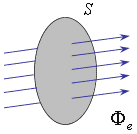
\includegraphics[width=0.45\textwidth]{images/image410.png}
				\caption{Поток излучения}
			\end{figure}
		}

	\end{frame}

	\begin{frame}{Геометрическая модель}
		\textbf{Поверхностная плотность потока энергии} $E_e$ --- величина потока~$\Phi_e$, приходящаяся на единицу площади $S$,
		\[
			E_e = \frac{\partial \Phi_e}{\partial S}, \qquad \bigg[ \frac{\text{Вт}}{\text{м}^2} \bigg]
		\]
		или 
		\textbf{энергетическая освещенность} $E_e$

		\vspace{0.15cm}

		Но также может быть наоборот.
		
		\textbf{Энергетическая светимость} $M_e$ --- поверхностная плотность потока энергии, излучаемая поверхностью.

		\note{

		В реальных условиях свет не равномерен, поэтому, в действительности, требуется интегрировать, чтобы учесть влияние освещенности на каждую точку поверхности

			\[
				\int E_e d S = \Phi_e
			\]
			или
			\[
				\int \int E_e d x d y = \Phi_e
			\]
			
			Таким образом,
			такой способ точно вычислить световой поток в общем случае, даже если освещенность распределена неоднородно по поверхности.
		}
	\end{frame}

	\begin{frame}{Обезразмеривание физических величин}
	
		Обезразмеривание физических величин --- процесс приведения уравнений или величин к безразмерному виду, то есть к форме, где отсутствуют явные единицы измерения. 
		Это достигается путём введения безразмерных переменных и масштабных величин. 

		\vspace{0.15cm}
		Выбор масштабных величин (характерных масштабов).

		Для начала необходимо определить характерные величины, которые будут использоваться для нормализации.\\
		% Эти величины обычно представляют собой параметры, характерные для системы, и их значения должны быть на физически разумном уровне.\\
		Эти величины должны быть выбраны таким образом, чтобы они описывали важнейшие аспекты системы.
		
		\footnotesize
		Например.\\

    $L_0$ --- характерная длина (например, радиус объекта или размеры области, где расположены все объекты);\\
    $T_0$ --- характерное время (например, время распространения волн);\\
    $U_0$ --- характерная скорость (например, скорость движения потока частиц).



		\note {
			Пример обезразмеривания модели освещения Ламберта.\\
			\[
			I = I_L k_d (\vec{L} \cdot \vec{N})
			,
			\]
			где
			$I$ — интенсивность отражённого света;
			$I_L$ — интенсивность источника;
			$k_d$ — коэффициент диффузного отражения;
			$\vec{L}$ — вектор направления на источник света;
			$\vec{N}$ — вектор нормали поверхности.
			
			Обезразмеривание:
			\begin{itemize}
					\item Нормализация интенсивности. $I' = \frac{I}{I_{\text{max}}}$, $I_L' = \frac{I_L}{I_{\text{max}}}$,
					\item Нормализация векторов $\vec{L}$ и $\vec{N}$ (обычно, уже нормализованы, т.е. $\|\vec{L}\| = \|\vec{N}\| = 1$).
			\end{itemize}
			
			Обезразмеренная модель имеет вид:
			\[
			I' = I_L' k_d (\vec{L} \cdot \vec{N}).
			\]
		}
	
	\end{frame}

	\begin{frame}{Телесный угол}{Solid angle}

		\textbf{Телесный угол} $\Omega$ (или твердый угол), измеряемый в стерадианах~(ср), представляет собой меру пространственного угла, измеряемого в трехмерном пространстве. \\
		Вычисляется как
		\[
			\Omega = \frac{S}{r^2}
			,
		\]
		где
		\(S\) --- площадь проекции поверхности;
		\(r\) --- радиус сферы.

		\vspace{0.15cm}

		Телесный угол определяется как соотношение площади проекции поверхности, заключенной между лучами, выпущенными из точки и пересекающими какой-то объект (обычно сферу), к квадрату радиуса этой сферы. \\

		Таким образом, телесный угол измеряет, насколько много пространства охватывает объект относительно точки наблюдения.

		\note{
			\begin{figure}
				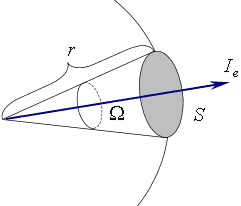
\includegraphics[width=0.45\textwidth]{images/image696.png}
				\caption{Телесный угол}
			\end{figure}
		}

	\end{frame}

	\begin{frame}{Угол и телесный угол}{Angle and Solid Angle}

		Рассмотрим следующие формулы
		\[
			d \theta = \frac{d L}{r}	
		,
		\]
		где
		\(d\theta\) --- изменение угла \(\theta\);
		\(dL\) --- изменение длины дуги;
		\(r\) --- радиус сферы.
		

		Следующая формула используется при интегрировании по сферической поверхности и является результатом преобразования элемента площади проекции поверхности \(dS\) в сферических координатах.
		\[
			d \Omega = \frac{dS}{r^2} 
			= 
			\frac{(r d \phi)(r \sin \theta d \theta)}{r^2} 
			= 
			\sin \theta  d \theta d \phi
			,
		\]
		где
		\(d\Omega\) --- элемент телесного угла;
		\(dS\) --- элемент площади проекции поверхности;
		\(r\) --- радиус сферы;
		\(d\theta\) --- элемент угла \(\theta\) (зенитного угла);
		\(d\phi\) --- элемент угла \(\phi\) (азимутального угла).
		

		\note{
			\begin{figure}
				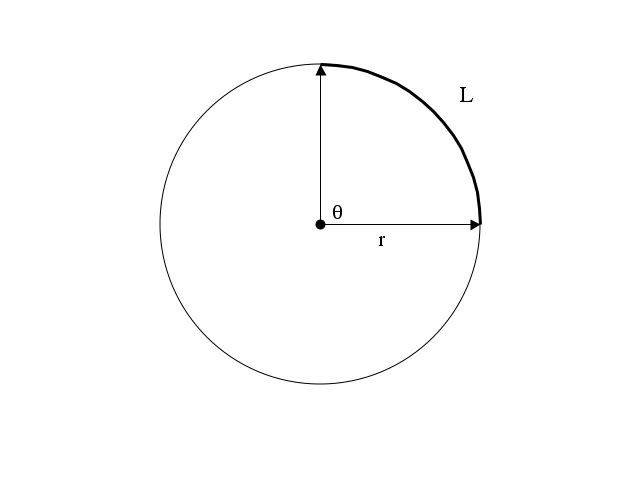
\includegraphics[width=0.45\textwidth]{images/radians.jpg}
				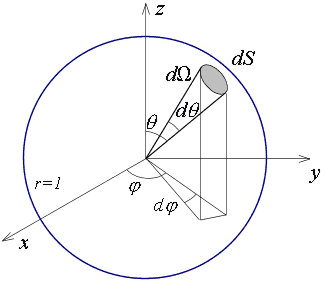
\includegraphics[width=0.45\textwidth]{images/solid_angle_2.png}
				\caption{Угол в полярных координатах (слева) и телесный угол в сферических координатах (справа)}
			\end{figure}
		}
	\end{frame}

	\begin{frame}{Площадь сферы}{Differential Solid Angles}
		Итак, телесный угол описывается следующей формулой
		\[
			d \omega = \frac{d S}{ r^2} =	\sin \theta  d \theta d \phi
		\]
		Площадь единичной сферы через телесный угол и в сферической системе координат
		\[
			S_\text{sphere} = \int_{\Omega} d \omega 
			= 
			\int_{0}^{2\pi}\int_{0}^{\pi} \sin \theta  d \theta d \phi
			= 
			\int_{0}^{\pi} \sin \theta d \theta \int_{0}^{2\pi} d \phi
			=
			4 \pi
		\]

		\note{
			\begin{figure}
				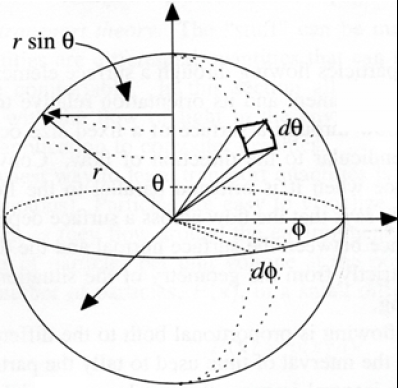
\includegraphics[width=0.55\textwidth]{images/sphere_surface.png}
				\caption{Схема расчета площади сферы}
			\end{figure}
		}
	\end{frame}

	\begin{frame}{Ракурс}{Foreshortening}
		Большой источник, рассмотренный под косым углом, должен создавать тот же эффект, что и маленький источник, расположенный перпендикулярно. Это явление известно как ракурс.

		\note{
			\begin{figure}
				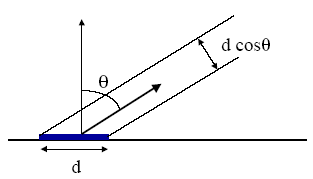
\includegraphics[width=0.75\textwidth]{images/foreshortening.png}
				\caption{Пример ракурса}
			\end{figure}
		}
	\end{frame}
	
	\begin{frame}{Расчет телесного угла}{Solid Angle Computing}
		
		Телесный угол $\omega$ --- мера пространства, определяемая проекцией заданной области поверхности на единичную сферу с центром в исходной точке.

		Телесный угол характеризует долю сферической поверхности, на которую проецируется рассматриваемая область.

		\[
			d \omega = d A_0 = \frac{d A \cdot \cos \theta}{ r^2}
		\]

		\note{
			\begin{figure}
				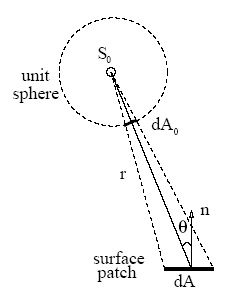
\includegraphics[width=0.4\textwidth]{images/solid_angle_.png}
				\caption{Схема расчета телесного угла}
			\end{figure}
		}
	\end{frame}



	\begin{frame}{Энергетическая яркость}{Radiance}
		Распределение света в пространстве зависит от положения и направления источников света (объектов, которые излучают свет), а также объектов, образующих сцену.

		Подходящей единицей измерения для оценки распределения света в пространстве является \textbf{энергетическая яркость} L
		\[
			L = \frac{\partial^2 \Phi_e}{\cos \theta \partial \omega \partial A}
			, \qquad 
			\bigg[ \frac{\text{Вт}}{ \text{ср} \cdot \text{м}^2} \bigg]  
			\equiv  
			\bigg[ \text{нит} \bigg]
			,
		\]
		\footnotesize
		где 
		$L$ --- энергетическая яркость (Radiance), описывает количество светового потока, излучаемого поверхностью в определенном направлении, на единичную площадку и в единичный угловой диапазон;
		$d^2 \Phi$ --- элемент светового потока (Flux) через малую площадку $dA$  в малом угловом диапазоне $d \omega$;
		$\cos \theta$ --- косинус угла между нормалью к поверхности и направлением, в котором измеряется энергетическая яркость;
		$dA$ --- элемент площади поверхности, через которую измеряется световой поток;
		$d \omega$ --- элемент углового диапазона, в пределах которого измеряется световой поток.
		
		\note{
			
			\begin{figure}
				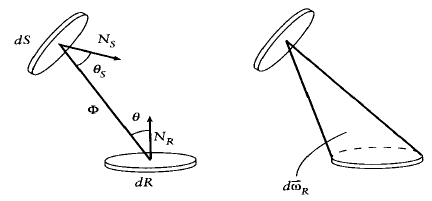
\includegraphics[width=0.9\textwidth]{images/radiance_ds_dr.png}
				\caption{Схема излучения из ds в dr}
			\end{figure}
		}

	\end{frame}

	\begin{frame}{Энергетическая яркость поверхности в конкретном направлении}
		Формула энергетической яркости поверхности в конкретном направлении
		% \[
		% 	d L = \frac{d^2 \Phi}{\cos \theta d \omega d A}
		% \] 
		\[
			L \cos \theta d \omega = \frac{d^2 \Phi}{ d A}
		\] 
		где 
		$L$ --- энергетическая яркость (Radiance), описывает количество светового потока, излучаемого поверхностью в определенном направлении, на единичную площадку и в единичный угловой диапазон ($W/(m²\cdot sr)$);
		$d^2 \Phi$ --- элемент светового потока (Flux) через малую площадку $dA$  в малом угловом диапазоне $d \omega$;
		$\cos \theta$ --- косинус угла между нормалью к поверхности и направлением, в котором измеряется энергетическая яркость;
		$dA$ --- элемент площади поверхности, через которую измеряется световой поток;
		$d \omega$ --- элемент углового диапазона, в пределах которого измеряется световой поток.
		
	\end{frame}

	\begin{frame}{Бесконечно маленький источник света и участки поверхности}

		Энергетическая яркость поверхности в точке x1 в направлении точки~x2 рассчитывается как
		% Radiance at x1 leaving to x2
		\[
			L(x_1,x_1 \to x_2) = 
			\frac{d \Phi}{d \omega \cos \theta_1 d A_1}
			=
			\biggl[ 
				d \omega = \frac{\cos \theta_2 d A_2 }{ r^2}
			\biggr]
			=
			\frac{r^2 d \Phi}{\cos \theta_2 d A_2   \cos \theta_1 d A_1}
		\]

		А в обратном направлении энергетическая яркость поверхности в точке x2 в направлении точки~x2 из точки~x1 рассчитывается как
		% Let the radiance arriving at x2 from the direction of x1 is
		\[
			L(x_2,x_1 \to x_2) = 
			\frac{d \Phi}{d \omega \cos \theta_2 d A_2}
			=
			\biggl[ 
				d \omega = \frac{\cos \theta_1 d A_1 }{ r^2}
			\biggr]
			=
			\frac{r^2 d \Phi}{\cos \theta_1 d A_1 \cos \theta_2 d A_2}
		\]

		\note{
			
		\begin{figure}
			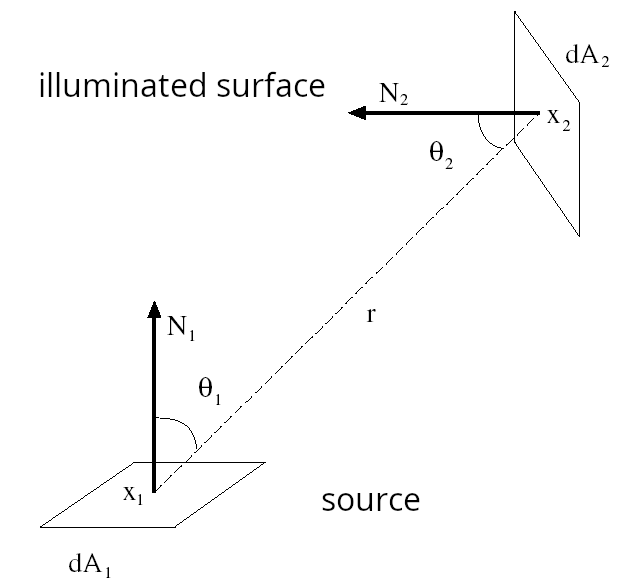
\includegraphics[width=0.6\textwidth]{images/radiance_ds_dr_.png}
			\caption{Излучение из ds в dr}
		\end{figure}
		
		}
	\end{frame}

	\begin{frame}{Расчет излученной энергии}{Computing Irradiance}

		Рассчитать входящую освещенность в точки $x$ для некоторой поверхности по заданной полусфере можно следующим образом:
		
		\[
			E(x) 
			= 
			\int_{\Omega_+} L(x, \omega_i) (n \cdot \omega_i) d \omega_i
			=
			\int_{0}^{2\pi}\int_{0}^{\pi / 2} 
			L(x, \theta_i, \phi_i) 
			\cos \theta_i 
			\sin \theta_i d \theta_i d \phi_i
		\]

	% Таким образом, излученная энергия из определенного направления составляет

	% \[
	% 	E(x) = L(x, \theta_i, \phi_i) \cos \theta_i  d \theta_i d \phi_i
	% \]



	\end{frame}

	\begin{frame}{Двулучевая функция отражательной способности}{Bidirectional Reflectance Distribution Function, BRDF}
		
		Двулучевая функция отражательной способности (ДФОС) описывает какая доля световой энергии, приходящей из одного направления, уходит в другом направлении для произвольной пары таких направлений. 
		
		Математически выражается следующим образом:
		% \[ \text{BRDF}(\theta_o, \phi_o, \theta_i, \phi_i) = \frac{\text{Исходящая яркость}(\theta_o, \phi_o)}{\text{Входящая интенсивность}(\theta_i, \phi_i)} \]
		% или

		\[
			%\text{BRDF}
			f_r (x, \theta_o, \phi_o, \theta_i, \phi_i) =
			% f(\theta_o, \phi_o,\theta_i, \phi_i) =
			\frac{d L(x, \theta_o, \phi_o)}{d E (x, \theta_i, \phi_i)}
			=
			f_r (x, \omega_o, \omega_i)
			=
			\frac{d L(x, \omega_o)}{d E (x, \omega_i)}
			% переписать знаменатель через L cos d w
		\]

		Здесь \(\theta_i\) и \(\phi_i\) представляют углы направления входящего света (обычно относительно нормали к поверхности), а \(\theta_o\) и \(\phi_o\) представляют углы направления исходящего света. 

		BRDF является фундаментальным концептом,
		% в компьютерной графике, компьютерном зрении и оптике, 
		предоставляя способ моделирования взаимодействия света с поверхностями и его отражения в различных направлениях.

		\note{
		\begin{figure}
			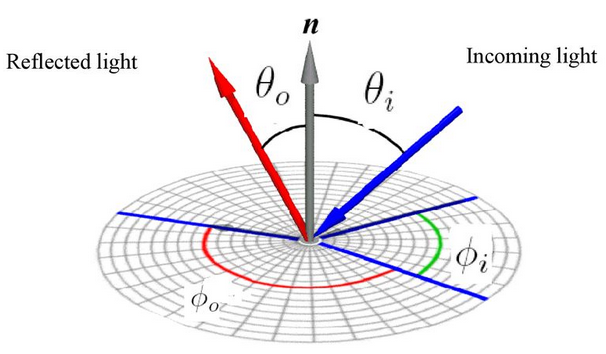
\includegraphics[width=0.8\textwidth]{images/brdf_2.png}
			\caption{Двулучевая функция отражательной способности}
		\end{figure}
		}
	\end{frame}

	\begin{frame}{}
		Излученность в направлении наблюдения при условии всех входящих световых потоков. 
		\[
			L(x, \theta_o, \phi_o) = 
			\int_{0}^{2\pi}\int_{0}^{\pi / 2}
			f_r(x, \theta_o, \phi_o, \theta_i, \phi_i) 
			L(x, \theta_i, \phi_i) 
			\cos \theta_i 
			\sin \theta_i d \theta_i d \phi_i
		\]
		или
		\[
			L(x, \omega_o) 
			=
			\int_{\Omega_+} 
			f_r(x, \omega_o, \omega_i) 
			L(x, \omega_i) 
			(n \cdot \omega_i)
			d \omega_i
		\]
		Что пропорционально яркости пикселя для этого луча.

		\note{ 
			\footnotesize
			Функция двустороннего распределения отраженного света (BRDF) обладает несколькими важными свойствами:

			1. Положительность. Значения BRDF обычно неотрицательны для всех углов входа и выхода света.
			
			2. Нормализация. Интеграл BRDF по всем направлениям входа и выхода света равен единице. Это свойство обеспечивает сохранение энергии в системе.
			
			3. Ротационная инвариантность. BRDF не зависит от ориентации координатной системы, т.е. она инвариантна относительно поворотов.
			
			4. Симметрия. BRDF симметрична относительно обмена направлений входа и выхода света (\(\theta_i, \phi_i\) и \(\theta_o, \phi_o\)).
			
			5. Локальная изотропия или анизотропия. BRDF может быть изотропной (не зависит от направления) или анизотропной (зависит от направления).
			
			6. Монотонность. Поверхности с монотонной BRDF не могут сосредотачивать свет.
			
			7. Микрогеометрическая зависимость. BRDF часто зависит от микрогеометрии поверхности (например, шероховатости или микронеровностей).
			
			% Эти свойства обеспечивают физически обоснованное и адекватное моделирование отражательных свойств различных материалов в компьютерной графике и графическом дизайне.

		}
	\end{frame}

	\begin{frame}{Световые и энергетические величины}
		\begin{table}
			\caption{\label{tab:fractal} Сравнение энергетических и световых величин}
			\begin{center}
				\renewcommand{\arraystretch}{1.5} 
				\begin{tabular}{|c|c|c|c|c|c|}
					\hline
					\multicolumn{3}{|c|} {Энергетические} & \multicolumn{3}{|c|} {Световые} \\
					\hline
					Поток излучения & $\Phi_e$ & Вт & Световой поток & $\Phi$ & лм \\
					\hline
					Энергетическая сила света & $I_e$ & $\frac{\text{Вт}}{\text{ср}}$ & Сила света & $I$ & кд \\
					\hline
					Энергетическая освещенность & $E_e$ & $\frac{\text{Вт}}{\text{м}^2}$ & Освещенность & $E$ & лк \\
					\hline
					Энергетическая светимость & $M_e$ & $\frac{\text{Вт}}{\text{м}^2}$ & Светимость & $M$ & $\frac{\text{лм}}{\text{м}^2}$ \\
					\hline
					Энергетическая яркость & $L_e$ & $\frac{\text{Вт}}{\text{cр}\cdot \text{м}^2}$ & Яркость & $L$ & $\frac{\text{кд}}{\text{м}^2}$ \\
					\hline
				\end{tabular}
			\end{center}
		\end{table}

		\footnotesize
		Примечание.
		Световой поток измеряется в лм (люменах) и представляет собой полную видимую энергию, излучаемую источником света за единицу времени.

		\note{

		\textbf{Люмен} (лм) измеряет световой поток, представляя собой общее количество света, излучаемого источником света в одну секунду; используется для оценки яркости светильников и ламп.

		\textbf{Кандела} (кд) измеряет световой поток в заданном направлении, представляя собой интенсивность света в конкретном угловом направлении; введена для оценки яркости источников света, особенно в направленных световых системах.

		\textbf{Люкс} (лк) измеряет освещенность, представляя собой количество света, падающего на поверхность в один люкс, равный одному люмену на квадратный метр; введен как метрика для оценки комфортного освещения.
		
		\vspace{0.15cm}

		\footnotesize

		Историческая справка. 
		Люкс и люмен стали стандартами измерения света в 20 веке, с развитием технологий освещения. В 1948 году была введена спецификация лм для измерения светового потока. Кандела была предложена в 1946 году в ходе разработки стандартов единиц измерения света, утвержденных в 1979 году.
		% https://novolampa.ru/baza-znaniy/kandely-lyuminy-lyuksy-v-chem-raznitsa/

		}
		
	\end{frame}

	\begin{frame}{Освещенность и светимость}
    Освещенность и светимость --- разные величины, связанные с освещением:

    \begin{itemize}
        \item \textbf{Освещенность} (\textit{E}) --- измеряет количество света, падающего на единицу площади.\\        
         Единица измерения: люкс (лм/м$^2$).\\
         Пример. лампа с потоком 1000 люмен освещает поверхность в 10 м², создавая освещенность 100 люкс.
        
        \vspace{0.5em}
        \item \textbf{Светимость} (\textit{M}) — характеризует общее количество света, излучаемого источником во всех направлениях.\\
         Единица измерения: люмен (лм).\\
         Пример. лампа с потоком 1000 люмен имеет светимость 1000 люмен.
        
    \end{itemize}

    \vspace{0.3em}
    \textbf{Разница}. Освещенность описывает свет на поверхности, а светимость --- общий свет, излучаемый источником.
	\end{frame}

	\begin{frame}{Заключение}
		Литература
		\begin{enumerate}
			\item \href{https://www.ece.lsu.edu/gunturk/EE4780/EE4780.html}{Bahadir K. Gunturk Radiometry, photometric stereo}
			\item \href{http://aco.ifmo.ru/el_books/basics_optics/glava-2/glava-2-1.html}{Родионов С.А. Основы оптики. Конспект лекций}
			\item Jinxiang C. Computer Graphics: Radiometry and Illumination 
			\item \href{https://novolampa.ru/baza-znaniy/kandely-lyuminy-lyuksy-v-chem-raznitsa}{Взаимосвязь силы света, светового потока и освещенности}
		\end{enumerate}

	\end{frame}
	
\end{document}